% Options for packages loaded elsewhere
\PassOptionsToPackage{unicode}{hyperref}
\PassOptionsToPackage{hyphens}{url}
\PassOptionsToPackage{dvipsnames,svgnames,x11names}{xcolor}
%
\documentclass[
  10pt,
]{article}
\usepackage{amsmath,amssymb}
\usepackage{iftex}
\ifPDFTeX
  \usepackage[T1]{fontenc}
  \usepackage[utf8]{inputenc}
  \usepackage{textcomp} % provide euro and other symbols
\else % if luatex or xetex
  \usepackage{unicode-math} % this also loads fontspec
  \defaultfontfeatures{Scale=MatchLowercase}
  \defaultfontfeatures[\rmfamily]{Ligatures=TeX,Scale=1}
\fi
\usepackage{lmodern}
\ifPDFTeX\else
  % xetex/luatex font selection
\fi
% Use upquote if available, for straight quotes in verbatim environments
\IfFileExists{upquote.sty}{\usepackage{upquote}}{}
\IfFileExists{microtype.sty}{% use microtype if available
  \usepackage[]{microtype}
  \UseMicrotypeSet[protrusion]{basicmath} % disable protrusion for tt fonts
}{}
\makeatletter
\@ifundefined{KOMAClassName}{% if non-KOMA class
  \IfFileExists{parskip.sty}{%
    \usepackage{parskip}
  }{% else
    \setlength{\parindent}{0pt}
    \setlength{\parskip}{6pt plus 2pt minus 1pt}}
}{% if KOMA class
  \KOMAoptions{parskip=half}}
\makeatother
\usepackage{xcolor}
\usepackage[margin=0.7in]{geometry}
\usepackage{longtable,booktabs,array}
\usepackage{calc} % for calculating minipage widths
% Correct order of tables after \paragraph or \subparagraph
\usepackage{etoolbox}
\makeatletter
\patchcmd\longtable{\par}{\if@noskipsec\mbox{}\fi\par}{}{}
\makeatother
% Allow footnotes in longtable head/foot
\IfFileExists{footnotehyper.sty}{\usepackage{footnotehyper}}{\usepackage{footnote}}
\makesavenoteenv{longtable}
\usepackage{graphicx}
\makeatletter
\def\maxwidth{\ifdim\Gin@nat@width>\linewidth\linewidth\else\Gin@nat@width\fi}
\def\maxheight{\ifdim\Gin@nat@height>\textheight\textheight\else\Gin@nat@height\fi}
\makeatother
% Scale images if necessary, so that they will not overflow the page
% margins by default, and it is still possible to overwrite the defaults
% using explicit options in \includegraphics[width, height, ...]{}
\setkeys{Gin}{width=\maxwidth,height=\maxheight,keepaspectratio}
% Set default figure placement to htbp
\makeatletter
\def\fps@figure{htbp}
\makeatother
\setlength{\emergencystretch}{3em} % prevent overfull lines
\providecommand{\tightlist}{%
  \setlength{\itemsep}{0pt}\setlength{\parskip}{0pt}}
\setcounter{secnumdepth}{-\maxdimen} % remove section numbering
\ifLuaTeX
  \usepackage{selnolig}  % disable illegal ligatures
\fi
\usepackage{bookmark}
\IfFileExists{xurl.sty}{\usepackage{xurl}}{} % add URL line breaks if available
\urlstyle{same}
\hypersetup{
  colorlinks=true,
  linkcolor={Maroon},
  filecolor={Maroon},
  citecolor={Blue},
  urlcolor={blue},
  pdfcreator={LaTeX via pandoc}}

\author{}
\date{}

\begin{document}

\section{Exact pole transport of the actual norm membership
remainder}\label{exact-pole-transport-of-the-actual-norm-membership-remainder}

2026-11-14. Lean source freeze
\texttt{23d78212afe6b379e51040abf66622305250f62b}. All claims unsigned
{[}pcc:unverified{]}.

The actual norm support and the full membership remainder now have exact
polynomial transport identities under the inverse-pair condition
\texttt{e*l=1}. They apply at every Dickson depth and imply an exact
coefficient normalization. The proof uses polynomial composition, norm
division and monic remainder uniqueness; it does not substitute
agreement on finite-field values for polynomial equality. Main unsigned
claims: remainder transport \texttt{PCC-20261114-d754b9} and coefficient
transport \texttt{PCC-20261114-9e7aa6} {[}pcc:unverified{]}.

\href{../lean/NormPoleTransport.lean}{Lean source},
\href{../POLE_TRANSPORT_PROTOCOL.md}{prospective contract},
\href{../pole-transport-evidence/claim-pins.json}{exact declaration
map}, \href{transport.dot}{editable diagram}, \href{transport.svg}{SVG},
\href{report.pdf}{report PDF}.

\begin{figure}
\centering
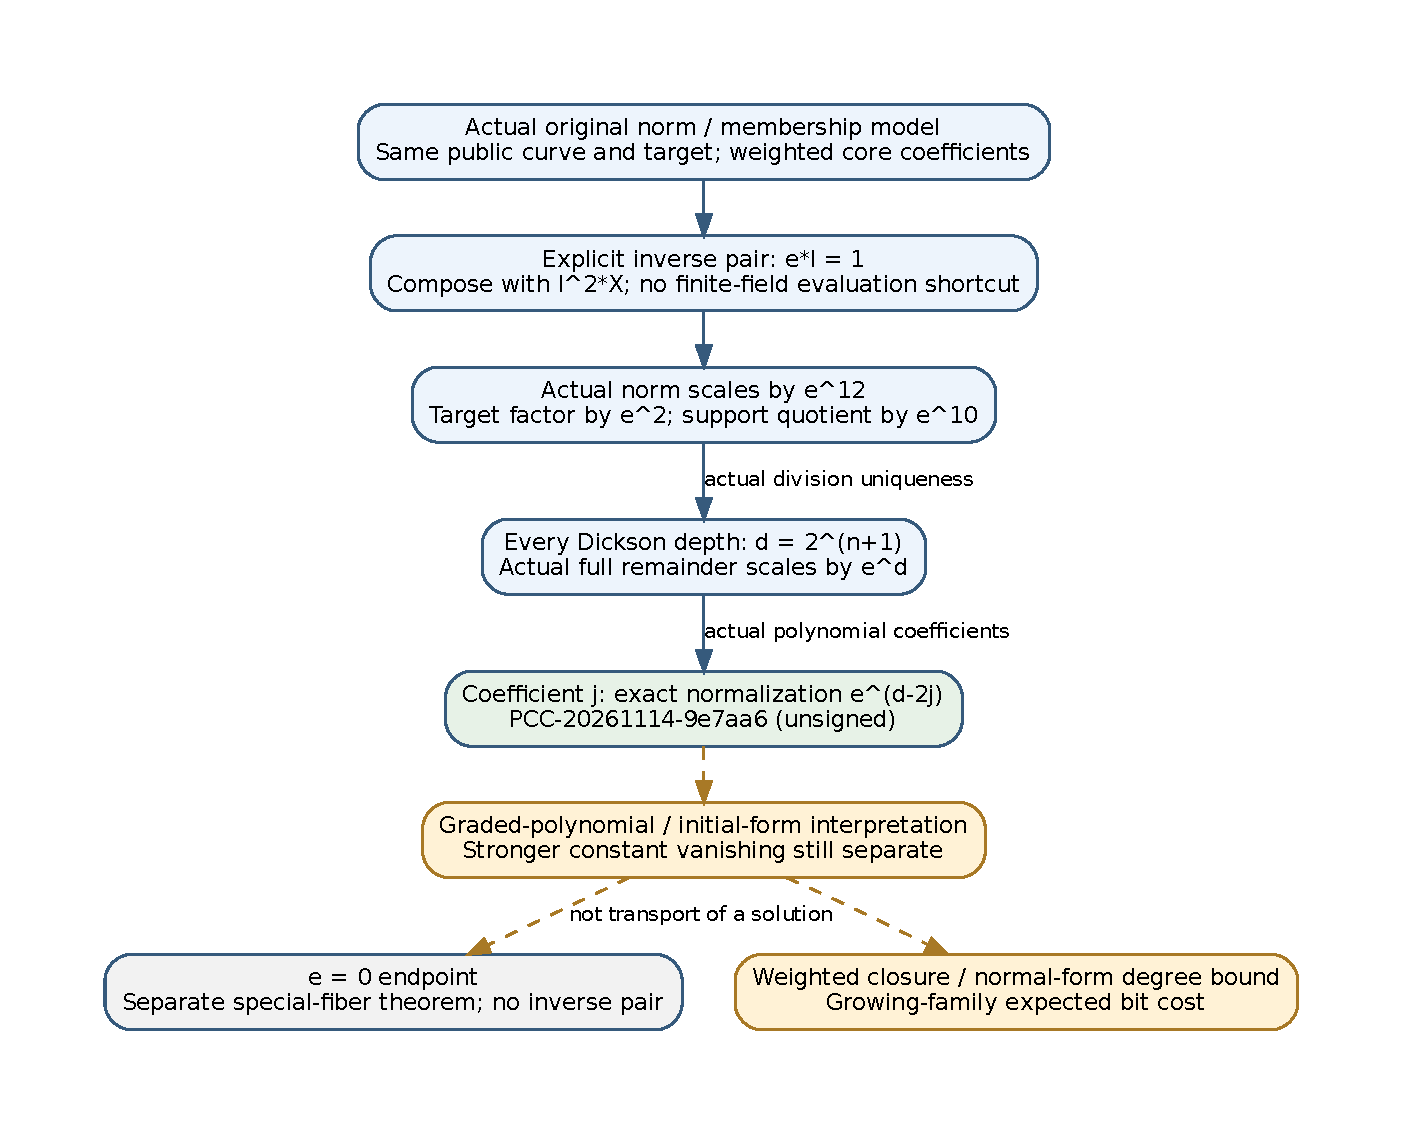
\includegraphics[width=0.9\textwidth,height=\textheight]{transport.pdf}
\caption{Exact invertible-parameter transport and the separate
graded/solver obligations. Solid arrows are source-bound Lean
identities; dashed arrows remain open. All evidence unsigned.}
\end{figure}

\subsection{Actual objects and the exact
map}\label{actual-objects-and-the-exact-map}

Over a field K, the original public target satisfies
\texttt{z\^{}2=r\^{}3+a*r+b}. The scalar and elementary polynomial
identities need only a commutative ring and an explicit inverse pair.
The actual source chart uses

\begin{verbatim}
D = X^3+a2*X^2+a1*X;  B = c0+c1*X
A = completeTarget(D,B,r,z) = D + z*B(r)-D(r)
N = A^2-(X^3+a*X+b)*B^2
U = N div (X-r)
P_n = master(2,n)-terminal;  R_n = P_n mod U.
\end{verbatim}

Target completion and the curve equation make norm division exact. The
actual support is monic degree5. These are constructed polynomials, with
no successful coefficient, divisor witness or solve oracle supplied. The
scalar functions are lifted through the actual constant-polynomial
homomorphism to actual univariate polynomials {[}pcc:unverified{]}.

Set \texttt{e*l=1}. Keep the original curve and target on the source
side, replace its four retained coefficients by

\begin{verbatim}
(a1*l^4, a2*l^2, c0*l^3, c1*l),  and compose with l^2*X.
\end{verbatim}

The completed A normalizes by \texttt{e\^{}6}, B by \texttt{e\^{}3}, and
the cubic by \texttt{e\^{}6}. Consequently the actual norm normalizes by
\texttt{e\^{}12}. The target factor normalizes by \texttt{e\^{}2}, so
the actual quotient normalizes by \texttt{e\^{}10}:

\begin{verbatim}
e^10 * U_original_scaled_core(l^2*X) = U_e.
\end{verbatim}

Here \texttt{U\_e} is exactly the existing
\texttt{NormWeightedLeading.scaledSupport}, with curve
\texttt{X\^{}3+e\^{}4*a*X+e\^{}6*b} and target
\texttt{(e\^{}2*r,e\^{}3*z)}. The quotient equation is derived from the
actual norm identity and monic division uniqueness, not assumed as a
transport premise in the main theorem. For j\textless=5, the coefficient
equation has normalization \texttt{e\^{}(10-2*j)} {[}pcc:unverified{]}.

At every depth n let \texttt{d=2\^{}(n+1)}. The actual Dickson
master-minus-terminal normalizes by \texttt{e\^{}d} to the existing
scaled master-minus-scaled-terminal. The full remainder then obeys the
polynomial identity

\begin{verbatim}
e^d * R_original_scaled_core(l^2*X) = R_e,n.
\end{verbatim}

For \texttt{2*j\textless{}=d}, taking coefficients gives

\begin{verbatim}
e^(d-2*j) * (R_original_scaled_core).coeff(j) = R_e,n.coeff(j).
\end{verbatim}

At depth4 the four nonconstant residuals have nominal normalization
exponents24,26,28,30 in descending X order. These are exact exponents in
the transport equation, not a measured degree profile or a solver bound.
The nominal constant exponent is32; its earlier predicted actual
weight30 requires a further graded vanishing/divisibility argument
{[}pcc:unverified{]}.

\subsection{Why the remainder proof is
substantive}\label{why-the-remainder-proof-is-substantive}

The generic remainder lemma assumes two monic degree5 moduli and the
exact unit/variable scaling relation between them. Its proof transports
the actual quotient/remainder equation. For any nonnegative
normalization exponent d, the new quotient is the old composed quotient
multiplied by \texttt{e\^{}d*l\^{}10}; this handles small depths without
a negative exponent. The transported remainder stays below degree5 by
the actual composition/scalar degree bounds. Monic division uniqueness
identifies it with the computed remainder. The actual norm support
theorem discharges the modulus-scaling premise in the main membership
theorem {[}pcc:unverified{]}.

For field-valued transport, the inverse pair excludes e=0. The previous
component separately computes that endpoint and proves its four
coefficient equations force the origin. No theorem transports the
special-fiber tuple to an original solution. At that endpoint the curve
equation is \texttt{y\^{}2=x\^{}3}; it is used for coefficient analysis,
without an elliptic-group transport assertion. The proof covers general
prime fields through its field hypotheses; no special curve, subgroup
order or hidden integer label is assumed {[}pcc:unverified{]}.

\subsection{Validation and construction
boundaries}\label{validation-and-construction-boundaries}

The module contains23 new statements and retains build receipts001--005,
including the failed full-tower drafts003--005, and final successful
build006. Only standard foundations occur in its axiom prints. The
whole-study gate reports327 statements,0 additional trusted uses, exit0;
import-inclusive fresh replay also exits0. Unsigned validation claim
\texttt{PCC-20261114-5a59a9} binds the
\href{../pole-transport-evidence/validation-001.json}{receipt}, exact
source/artifact hashes and preserved failures. The canonical adapter
has22 passing tests; format/build/issuance pass, with4 inherited
unchanged SHA256 strict-clippy style failures. All25 new source/data
claims remain unsigned; default-PATH verdicts are \texttt{not\_covered}
(exit2). Dependency pins remain Lean4.35.0, CryptoLean revision
\texttt{148f5dc389b341401e06d76abe7783c4ccf42f2e}, and Mathlib revision
\texttt{cfc55fc58714a59dc06e6e79edc6d1d95140d3c2}. These are the
preceding component's unchanged dependency revisions
{[}pcc:unverified{]}.

The separate canonical identity driver seals only this unconditional
intermediate ring step:

\begin{verbatim}
e^12*(A^2-F*B^2) = (e^6*A)^2-(e^6*F)*(e^3*B)^2.
\end{verbatim}

Certificate \texttt{IDC1h504690879b070928}, unsigned claim
\texttt{PCC-20261114-c8beeb}, has syntactic degree15 and32 statement-
derived plus16 extra replay points. It does not encode the inverse-pair
condition or the polynomial/remainder transport, and supplies no signed
execution evidence. The unchanged canonical adapter's checks and its
inherited SHA256 strict-clippy failures are retained separately
{[}pcc:unverified{]}.

No native fixture experiment, random sample, root/branch search,
F4/msolve, paid/cloud/attack run or performance comparison was attempted
here. Flow for the earlier fixed native fixture experiment remains1
planned,0 attempted, 0 completed,0 excluded,1 admission-blocked by
checkpoint upload. This component is universal mathematical
proof/certificate construction. The old benchrec1680/162 diagnostic
remains untouched, along with all earlier source, evidence, claims,
ledger bytes and compiler failures {[}pcc:unverified{]}.

\subsection{Sources checked and remaining
obligations}\label{sources-checked-and-remaining-obligations}

Sources checked (KB): same unavailable tools/wrapper as already
recorded; no unchanged failed retry. Reuse the bounded
\href{../weighted-leading-evidence/prior-search-receipt.json}{prior
review}, the actual old norm/scaledSupport/scaledMaster definitions, and
pinned Mathlib Polynomial.Eval.Degree \texttt{comp\_C\_mul\_X\_coeff},
composition identities, Polynomial.Div monic uniqueness, and the actual
degree lemmas used in source. These standard operations are reused
without a novelty/absence claim {[}pcc:unverified{]}.

The next proof is the graded-polynomial interpretation of these exact
invertible identities, including any stronger constant-coefficient
vanishing. An initial-ideal equality and a weighted
normal-form/iterated-closure bound remain open. Establishing those
bounds for a growing family and pricing finite-field extraction, yield,
relation collection and all expected bit costs remains necessary for the
broader goal. Input normalization alone does not supply such a bound
{[}pcc:unverified{]}.

The original W-jet family still needs its own public-input map. This
proof does not identify it with the norm-membership family. Global
performance scoreboard/timeline and curve graphs remain unchanged: no
measured speed or certified group transport edge was added. The earlier
study-local initial- form diagram also remains valid: the exact
invertible scaling map here strengthens its algebraic foundation while
its graded/solver arrows remain unresolved {[}pcc:unverified{]}.

\subsection{Exact proof map}\label{exact-proof-map}

Exact hypotheses and source binding hashes are in claim-pins.json. Every
claim is unsigned {[}pcc:unverified{]}.

\begin{longtable}[]{@{}ll@{}}
\toprule\noalign{}
NormPoleTransport declaration & Unsigned claim \\
\midrule\noalign{}
\endhead
\bottomrule\noalign{}
\endlastfoot
\texttt{inversePowers} & \texttt{PCC-20261114-f5b06b} \\
\texttt{completedValueScale} & \texttt{PCC-20261114-55d16a} \\
\texttt{branchValueScale} & \texttt{PCC-20261114-367118} \\
\texttt{curveValueScale} & \texttt{PCC-20261114-00cb72} \\
\texttt{normValueScale} & \texttt{PCC-20261114-9a26b0} \\
\texttt{completedValuePolynomial} & \texttt{PCC-20261114-e99a16} \\
\texttt{actualAComp} & \texttt{PCC-20261114-4b131c} \\
\texttt{actualAPoleScale} & \texttt{PCC-20261114-16801b} \\
\texttt{branchPoleScale} & \texttt{PCC-20261114-eb3429} \\
\texttt{curvePoleScale} & \texttt{PCC-20261114-255b47} \\
\texttt{normPoleScale} & \texttt{PCC-20261114-136a79} \\
\texttt{targetFactorPoleScale} & \texttt{PCC-20261114-f5a15d} \\
\texttt{masterPoleScale} & \texttt{PCC-20261114-6857b8} \\
\texttt{terminalPoleScale} & \texttt{PCC-20261114-cabd66} \\
\texttt{actualSupportExact} & \texttt{PCC-20261114-769bd6} \\
\texttt{supportPoleScale} & \texttt{PCC-20261114-97225a} \\
\texttt{supportCoefficientScale} & \texttt{PCC-20261114-351787} \\
\texttt{supportNormalizedCoefficient} & \texttt{PCC-20261114-955e02} \\
\texttt{actualSupportWindow} & \texttt{PCC-20261114-4fec47} \\
\texttt{scaledSupportWindow} & \texttt{PCC-20261114-88a657} \\
\texttt{remainderPoleScale} & \texttt{PCC-20261114-0750e7} \\
\texttt{membershipPoleScale} & \texttt{PCC-20261114-d754b9} \\
\texttt{membershipCoefficientScale} & \texttt{PCC-20261114-9e7aa6} \\
\end{longtable}

\end{document}
